\documentclass{report}


\usepackage{pdfpages}

\usepackage{color} %red, green, blue, yellow, cyan, magenta, black, white
\definecolor{mygreen}{RGB}{28,172,0} % color values Red, Green, Blue
\definecolor{mylilas}{RGB}{170,55,241}

\usepackage{listings}
\usepackage{caption}
\usepackage{subcaption}
\usepackage{hyperref}
\hypersetup{%
  colorlinks=false,% hyperlinks will be black
%  linkbordercolor=red,% hyperlink borders will be red
  pdfborderstyle={/S/U/W 1}% border style will be underline of width 1pt
}


\usepackage{graphicx}
\usepackage{fancyhdr}
\pagestyle{fancy}
\fancyhf{}
\lhead{}
\chead{\textsl{Hexapod Robot}}
\rhead{}
\lfoot{\textsl{Department Of Electronics,CE Cherthala}}
\rfoot{\thepage}

\renewcommand{\headrulewidth}{2pt}
\renewcommand{\footrulewidth}{2pt}

\fancypagestyle{plain}{%
\fancyhf{}%
\lhead{}%
\chead{\textsl{Hexapod Robot}}%
\rhead{}%
\lfoot{\textsl{DoE,CE Cherthala}}%
\rfoot{\thepage}%

\renewcommand{\headrulewidth}{2pt}%
\renewcommand{\footrulewidth}{2pt}}

\usepackage{titlesec}
\renewcommand{\chaptername}{CHAPTER}
\titleformat{\chapter}[display]
  {\normalfont\sffamily\Large\bfseries\centering}
  {\chaptertitlename\ \thechapter}{0pt}{\Huge}
\titleformat{\section}
  {\normalfont\sffamily\large\bfseries}
  {\thesection}{1em}{}
\titlespacing*{\chapter}{0pt}{30pt}{20pt}

% tikz package defeninition starts
\usepackage{tikz}

\newcommand*{\DashedArrow}[1][]{\mathbin{\tikz [baseline=-0.25ex,-latex, dashed,#1] \draw [#1] (0pt,0.5ex) -- (1.3em,0.5ex);}}%

\usetikzlibrary{calc}
\usetikzlibrary{shapes.geometric, arrows}
\tikzstyle{line}=[draw,-latex'] 
\tikzstyle{box} = [rectangle, rounded corners, minimum width=2cm, minimum height=2cm,text centered,thick, draw=black,text width=1.8cm]
\tikzstyle{gui} = [ellipse,draw=black, fill=red!10,minimum height=1cm]


\tikzstyle{arrow} = [thick,->,>=stealth,label=above]


% For flowcharts

\tikzstyle{line}=[draw,-latex'] 
\tikzstyle{startstop} = [rectangle, rounded corners, minimum width=3cm, minimum height=1cm,text centered, draw=black, fill=blue!10]

\tikzstyle{io} = [trapezium, trapezium left angle=70, trapezium right angle=110, minimum width=3cm, minimum height=1cm, text centered, draw=black, fill=blue!10]

\tikzstyle{process} = [rectangle, minimum width=3cm, minimum height=1cm, text centered, text width=5cm, draw=black, fill=blue!10]

\tikzstyle{decision} = [diamond, minimum width=3cm, minimum height=1cm, text centered,text width=2cm, draw=black, fill=blue!10]

\tikzstyle{arrow} = [thick,->,>=stealth]


%tikz end



\definecolor{mygreen}{rgb}{0,0.6,0}
\definecolor{mygray}{rgb}{0.5,0.5,0.5}
\definecolor{mymauve}{rgb}{0.58,0,0.82}

\begin{document}



% LISTINGS DEFENITION STARTS
\lstset{ %
  backgroundcolor=\color{gray!10},   % choose the background color; you must  add \usepackage{color} or \usepackage{xcolor}
%  basicstyle=\footnotesize,        % the size of the fonts that are used for the code
  breakatwhitespace=false,         % sets if automatic breaks should only happen at whitespace
  breaklines=true,                 % sets automatic line breaking
  captionpos=b,                    % sets the caption-position to bottom
  commentstyle=\color{mygreen},    % comment style
  deletekeywords={...},            % if you want to delete keywords from the given language
  escapeinside={\%*}{*)},          % if you want to add LaTeX within your code
  extendedchars=true,              % lets you use non-ASCII characters; for 8-bits encodings only, does not work with UTF-8
%  frame=single,                    % adds a frame around the code
  keepspaces=true,                 % keeps spaces in text, useful for keeping indentation of code (possibly needs columns=flexible)
  keywordstyle=\color{blue},       % keyword style
  language=C,                 % the language of the code
  morekeywords={*,...},            % if you want to add more keywords to the set
  numbers=none,                    % where to put the line-numbers; possible values are (none, left, right)
  numbersep=5pt,                   % how far the line-numbers are from the code
  numberstyle=\tiny\color{mygray}, % the style that is used for the line-numbers
  rulecolor=\color{black},         % if not set, the frame-color may be changed on line-breaks within not-black text (e.g. comments (green here))
  showspaces=false,                % show spaces everywhere adding particular underscores; it overrides 'showstringspaces'
  showstringspaces=false,          % underline spaces within strings only
  showtabs=false,                  % show tabs within strings adding particular underscores
  stepnumber=2,                    % the step between two line-numbers. If it's 1, each line will be numbered
  stringstyle=\color{mymauve},     % string literal style
  tabsize=2,                       % sets default tabsize to 2 spaces
%  title=Program 3.2: Interrupt Subroutine                   % show the filename of files included with \lstinputlisting; also try caption instead of title
%caption = Interrupt Subroutine
}


%%LISTINGS DEFENITION ENDS




\title{\bfseries HEXAPOD ROBOT}
\author{Sarath.M}
\date{\today}
\maketitle
\chapter*{ACKNOWLEDGMENTS}
\pagenumbering{roman}
This major project has been possible only due to support and help from various people. This report would not complete unless their contributions are acknowledged.

	First of all, we would like to thank \textbf{Dr.Suresh Kumar, Principal, College Of Engineering,Cherthala} and to the management of College of Engineering,Cherthala for giving us an opportunity and encouragement to do this work. We would like to express our sincere thanks to \textbf{Mr.Pradeep M, Head of the Department of Electronics and Communication,College of Engineering, Cherthala} for giving timely support he gave whenever required. We express our profound gratitude to \textbf{Mrs.Ajay Nath S.A, Assistant professor} for his help, inspiration, guidance, suggestions, cooperation and innovative ideas.

We wish to express our sincere gratitude to our major project coordinators \textbf{Mr.Sreekumar.K, Assistant professor} for his guidance and timely help rendered. Also, we would like to express our thanks to \textbf{Mrs Subeena Subair} and \textbf{Mr Vishnu Pradeep K}; Assistant Professors, EC Department, for their valuable help and guidance. Last but certainly not the least we would like to express our gratitude to our family and friends, for their unending support, love and encouragement.


\chapter*{ABSTRACT}
Agriculture is big business. But the future of big farming isn’t in massive machinery, but swarms of smart, cheap 'bots seeding, tending and harvesting fields one plant at a time. Whether conducted by an industrial farming outfit or a small, independent farmer, agriculture is all about yield. Per-acre production makes or break the year, and taken at the macro level it impacts global markets and can lead to humanitarian crises. And while agriculture already happens at the field-by-field level,we can improve the profit margin \& the net productivity if we make agriculture even more precise. Think: plant-by-plant farming, optimized on a seed-by-seed basis.
But to manage such a precise, immense workload we need autonomous robots.\\
Keeping this in mind we have tried to develop hexapod walking robots; a six‐legged walking robot that is capable of basic mobility tasks such as
walking forward, backward, rotating in place which can be used in the field of agriculture.
The legs will be of a modular design. This robot will serve as a platform onto which additional sensory components could be added, or which could be programmed to perform increasingly complex motions.\\
The design presented in this report makes use of two simple revolute joints per leg and the required motion is provided by DC Servo motors. These 2 degrees of freedom will propel the robot in the direction of motion.
%\listoftables
\listoffigures
\tableofcontents

\chapter{PROBLEM STATEMENT}
\pagenumbering{arabic}
\section{Introduction}
\subsection{General Aspects}
For many years robotic systems have been widely used for industrial production and in warehoues, where a controlled environment has been a vision initiated in the early 1960's with basic research on projects on projects on automated steered systems and autonomous tracters. Recently , the developement of robotic systems in agriculture has experienced an increased interest , which has led many experts to explore the possibilities to develop more rational and adaptabe vehicles based on a behavioral approach.\\
In the open and outdoor environment, which will be the focus here , robotic and autonomous systems are more complex to develop - mainly because of safety issues . The robots safety system would have to be reliable enough for it to operate autonompously and unattended . It is relatively costly to develop safety systems if the vehicle has to be completely autonomous. In principle, they can work 24 hours a day but if a robot has to be attended then the time is limited by the person. In this matter, different scenarios and degrees for autonomy have been investigated depending on the task to be carried out.\\
The vehicles should be able to carry out useful tasks all year around, unattended and able to behave sensibly in a semi-natural environment over long periods of time. The small vehicles may also have less environmental imapct replacing the over- application of chemicals,and fertilisers , requires lower usage of energy with better control matched to requirements, as well as causing less soil compaction due to lighter weight.
\subsection{Economics}
Goense (2003) compared autonomous with conventional vehicles, equipped with implements having working
widths from 50 to 120 cm. He showed that if an autonomous vehicles can be utilised 23 hours a day, it would
be economic feasible with slight reductions in prices of navigation systems or with slight increases in labour
costs. Goense also discussed a number of other changes that will effect the final result, such as the fraction
of labour time needed out of the total machine time and the machine tracking system, which provides better
utilisation of machine working width and there is no need for operators rest allowance. On the other hand,
there may be negative effects in the form of higher costs in travelling distances for service personal.
\section{Areas Of Application}
\subsection{Crop establishment}
For traditional crop establishment and seed bed preparation it has been common that the whole topsoil of a
eld is inverted with a plough to create a suitable seed bed. This is a well known operation that suits many
circumstances but it also uses a lot of energy.
If the same seed environment can be achieved by only mixing the soil within a few centimetres of the actual
seed then the rest of the soil does not need to be disturbed as it can be well conditioned by natural soil 
ora
and fauna.\\
Another traditional concept is to grow crops in rows. It would seem that the only explanation as to why this
is done is that it requires the simplest type of machines. Seeds are placed relatively densely along each row.
The problem is that in principle, each plant requires equal access to light, air, water and nutrients, which
are often spatially related. Intra crop competition can be reduced by giving a more even or equal spacing
and seed distribution with accurate placement of seeds in a more uniform pattern.\\
If the location of each seed is known and the position of each emerged crop plant is estimated, it will be possible to identify each plant by its spatial location. Improved information about plant characteristics allows improved management and decision making and allows a numbe of improved, more targeted operations that can improve the overall crop efficiency.\\
As only a small volume of soil is needed to be cultivated there are a number of different methods that could be used. Rotary mechanical tillage in two dimensions on a vertical or horizontal axis could be used instead of just one dimension or water-jetting or the use of a hygroscopic polymer gel could be used to create a micro climate for the seed.
\section{Crop scouting}
An important part of good management is the ability to collect timely and accurate
information about the crop development. Quantified data has tended to be expensive and
sampling costs can quickly out weigh the benefits of spatially variable management.
(Godwin et al., 2003).\\
Data collection would be less expensive and timelier if an automated system could remain
within the crop canopy for continual monitoring that can be used for assessing crop status.
This could be achieved by either embedding cheap wireless sensors at strategic positions
within the crop, or placing more expensive sensors onto a moving platform.\\
With the advent of biosensors, a whole new set of opportunities will become available to
monitor growing crops for pest and disease attack (Tothill, 2001). As the
robotic/autonomous vehicle could patrol the fields continually looking for weeds and other
threats, real-time alerts could be sent to the manager whenever certain conditions were
encountered. These could take the form of noting actual pest or disease attack or by
monitoring environmental conditions where they are likely to occur or that the risk of attack
is significant. Differing growth rates could also be used to identify potential problems.
\subsection{Selective harvesting}
At present, crops are usually harvested when the average of the whole field is ready as this
simplifies the harvest process. Selective harvesting involves the concept of only harvesting
those parts of the crop that meet certain quantity or quality thresholds. It can be considered
to be a type of pre sorting based on sensory perception. Selective harvesting has been well
known in forestry for many years where certain trees are harvested according to quality and
size or to improve the quality of the remaining trees.\\
In agriculture, examples could be to only harvest barley below a fixed protein content or
combine grain that is dry enough (and leave the rest to dry out) or to select and harvest
fruits and vegetables that meet a size criteria.
As these criteria often attract quality premiums, increased economic returns could justify the
additional sensing.\\
Most agricultural vehicles are getting bigger and hence not suited for this approach. Therefore, smaller and
more versatile selective harvesting equipment is needed for this purpose. Either the crop can be surveyed
before harvest so that the information needed about where the crop of interest is located, or that the harvester may have sensors mounted that can ascertain the crop condition. The selective harvester can then harvest that crop that is ready, while leaving the rest to mature, dry, or ripen etc.\\
As the products are already graded or sorted, it also adds value to the products before they leave the farm.
\section{Target specifications of feasible solution}
We need a robot configuration that is suitable for farm environment. Our next step was to find such a system.\\
We found out that for an outdoor environment legged robots where more promising compared to wheeled robots due to  reasons as explained in next section
\subsection{Reasons to choose legged configuration}
Wheeled vehicles excel when used on prepared surfaces , such as roads and railways. They are cost-effective, efficient and capable of achieving higher velocities than any legged vehicle. However as the terrain becomes increasingly difficult, a point comes where wheeled vehicles prove inferior to legged vehicles.\\
Paddy fiels, sandy soils, and undulating terrain are troublesome for wheeled robots to cross; and specifically, that travelling over undulating natural terrains involves difficult tasks for wheeled vehicles, such as step climbing , gap crossing gradients, side slopes and water crossing\\
Similarly traversing many man-made terrains is also difficult for wheeled robots  because of narrow doorways, narrow hallways, sharp turns, floor irreglarities, ramps,raps, steps, staircase and ladders\\
When traversing soft soils, wheels sink down and must effectively be continuously climbing out of a hole and/or expending energy to compact the soil (See fig. ~\ref{fig1}). Foots most fundamental advantage over the wheel is that the compaction resistance of the soil can contribute to its forward thrust, whereas in the case of a wheel, compaction resistance reduces the forward thrust.
\begin{figure}[h!]
\centering
\includegraphics[width=\textwidth]{figcompaction}
\caption{Compaction Resistance of a wheel in soft soil}
\label{fig1}
\end{figure}
\subsection*{Other advantages of legged configuration}
\begin{enumerate}
\item Higher speed
\item Better fuel economy
\item Greater mobility (This includes the ability to step over obstacles and travel across terrain that is impossible for wheeled and tracked vehicles)
\item Better isolation from terrain irregularities. (This enables a smoother ride)
\item Less environmental damage. (Wheeled and tracked vehicles leave continuous ruts in soft soils, whereas legged vehicles leave only distinct footprints)
\end{enumerate}
In general, legged vehicles become attractive for applications requiring traversal of terrain that is too difficult for wheeled and tracked vehicles.   
\subsection{Legged robots}
Legged robots can be classified based on the number of legs used. They are :\\
\begin{itemize}
\item One legged: \emph{Hopper robot}
\begin{figure}[h!]
\centering
\includegraphics[scale=0.5]{p2}
\caption{Toyota Monoped}
\label{fig12}
\end{figure}   
\item Two legged robots: \emph{Biped robot}
\begin{figure}[h!]
\centering
\includegraphics[scale=0.5]{p3}
\caption{Honda ASIMO robot}
\label{fig13}
\end{figure}   
\item Three or more legged robot\\ 
\begin{figure}[h!]
\centering
\includegraphics[scale=0.5]{p4}
\caption{Boston Dynamic BigDog}
\label{fig14}
\end{figure}
\linebreak 
\item Hexapod
\begin{figure}[h!]
\centering
\includegraphics[scale=0.5]{p5}
\caption{model of the Hexapod}
\label{fig15}
\end{figure}   
\end{itemize}
 Out of these configurations we choose the Hexapod configuration due to reasons explained in the next section
 \subsection*{Reasons for choosing six-legged Hexapod configuration}
Hexapod robots have a large number of real life applications, from crossing potentially dangerous terrain to carrying out search and rescue operations in hazardous and unpredictable disaster zones. They have a number of advantages over wheeled, quadruped or bipedal robots:\\
\begin{itemize}
\item While wheeled robots are faster on level ground than legged robots, hexapods are the fastest of the
legged robots, as they have the optimum number of legs for walking speed - studies have shown
that a larger number of legs does not increase walking speed (Alexadre et al, 1991).
\item Having maneuverable legs allows hexapods to turn around on the spot
\item In comparison to other multi-legged robots, hexapods have a higher degree of stability as there are can be up to 5 legs in contact with the ground during walking. Also, the robots center of mass stays consistently within the tripod created by the leg movements, which also gives great stability
\item Hexapods also show robustness, because leg faults or loss can be managed by changing the walking
mechanism
\item This redundancy of legs also makes it possible to use one or more legs as hands to perform dexterous
tasks
\end{itemize}
\chapter{CIRCUIT LEVEL DESCRIPTION}
\section{Components list}
The various components used in the project are:

\begin{itemize}
\item DC Servo Motors
\item PIC16F877a
\item ZIGBEE module
\item Wireless Camera
\item DAGU Hexapod Chasis
\item Sensors
\begin{enumerate}
\item Temperature Sensor
\item Humidity Sensor
\item IR Senso
\end{enumerate}
\end{itemize}

\subsection*{\emph{DC Servo motor}}
It is a Hitec HS-645MG High torque. The running current is 450mA and the idle current is 9.1mA with an operating voltage 4.8 volt or 6 volt.
\begin{figure}[h!]
\centering
\includegraphics[scale=0.5]{fig31}
\caption{Hitec HS-645MG servo motor}
\label{fig21}
\end{figure}
\subsection*{\emph{PIC 16f877a}}
PIC 16F877 is one of the most advanced microcontroller from Microchip. This controller is widely used for experimental and modern applications because of its low price, wide range of applications, high quality, and ease of availability. It is ideal for applications such as machine control applications, measurement devices, study purpose, and so on.  The PIC 16F877 features all the components which modern microcontrollers normally have. Fig ~\ref{fig22} show the DIP package of PIC 16f877a
\begin{figure}[h!]
\centering
\includegraphics[scale=0.5]{fig32}
\caption{PIC 16f877a}
\label{fig22}
\end{figure} 
\subsection*{\emph{Wireless Camera kit}}
This is a 2.4GHz 4CH wireless mini camera kit including a wireless CMOS camera with MIC function and a wireless receiver. Easy installation and operation is suitable for home security. The frequency of the camera is fixed, by default is 2414 Mhz.
\begin{figure}[h!]
\centering
\includegraphics[scale=0.25]{fig34.jpg}
\caption{Wireless Camera kit}
\label{fig23}
\end{figure}
\subsection*{\emph{ZIGBEE modules}}
ZigBee is a specification for a suite of high level communication protocols used to create personal area networks built from small, low-power digital radios. ZigBee is based on an IEEE 802.15 standard. Though low-powered, ZigBee devices can transmit data over long distances.
\begin{figure}[h!]

\begin{subfigure}{0.5\textwidth}
	\centering
	\includegraphics[scale=0.25]{fig33a.jpg}
\caption{ZIGBEE Pro}
\end{subfigure}%
%
\begin{subfigure}{0.5\textwidth}
	\centering
	\includegraphics[scale=0.2]{fig33b}
	\caption{ZIGBEE usb dongle}
\end{subfigure}

\caption{ZIGBEE transmitter and receiver}
\label{fig24}
\end{figure} 
\subsection*{\emph{Hexapod robot chassis}}
This is a hexapod robot chassis that comes with 12 servos. It is made of acrylic with rubberized foam feet. This chassis was purchased online from Rhydolabz and was used for building the first prototype.
\begin{figure}[h!]
\begin{subfigure}{0.5\textwidth}
	\centering
	\includegraphics[scale=0.14]{chassis.jpg}
\caption{Chassis parts}
\end{subfigure}%
%
\begin{subfigure}{0.5\textwidth}
	\centering
	\includegraphics[scale=0.5]{dagu}
	\caption{after setting up}
\end{subfigure}
\caption{Hexapod chassis}
\label{fig25}
\end{figure}          
\subsection*{\emph{Sensors:}}
\subsubsection{Temperature sensor}
This is the latest DS18B20 1-Wire digital temperature sensor from Maxim IC. Reports degrees C with 9 to 12-bit precision, -55C to 125C (+/-0.5C)
\begin{figure}[h!]
\centering
\includegraphics[scale=0.5]{ds1820}
\caption{DS 1820 temperature sensor}
\label{fig26}
\end{figure}
\FloatBarrier

\subsubsection{Humidity sensor}
 This sensor module converts relative humidity(30-90\% RH) to voltage and can be used in weather monitoring application.
\begin{figure}[h!]
\centering
\includegraphics[scale=0.5]{humidity.jpg}
\caption{SY-HS-220 Humidity sensor}
\label{fig27}
\end{figure}
\subsubsection{Infrared proximity sensor}
Infrared proximity sensor made by Sharp. Part \#  GP2Y0A21YK has an analog output that varies from 3.1V at 10cm to 0.4V at 80cm. The sensor has a Japanese Solderless Terminal (JST) Connector. 
\begin{figure}[h!]
\centering
\includegraphics[scale=0.255]{ir.jpg}
\caption{Proximity sensor - Sharp GPY2Y0A21YK}
\label{fig28}
\end{figure}
\section{Circuit Diagram}
The main circuit is split into various blocks and explained in the following sections.
\subsection{PIC 16f877a and it's interface circuit}
The above circuit shows PIC16F877A MC and its corresponding interface circuit. The X1 crystal and the capacitors C1 and C2 are used to generate the 20 MHz clock signal to the microcontroller.

The push button which is pulled down to ground by a 10k resistor R1 acts as the reset button for the MC

The IO pins RB1-RB7 and RD1-RD7 are used as control pins for 13 servo motors(12 legs+head servo).

RA3 is connected to the signal pin of IR sensor(pin 2). The signal value of pin2.

The zigbee is connected to pins 25 and 26 of PIC. Wherte 25 is the Tx pin and pin 26 is the Rx pin of the PIC IC\\
\begin{figure}[h!]
\centering
\includegraphics[scale=0.8]{circpic}
\caption{PIC 16f877a}
\label{fig29}
\end{figure}
\subsection{ZIGBEE module and it's interface circuit}
The circuit diagram shown below is the interface circuit of zigbee using darlington pair.

The Darlington transistor (often called a Darlington pair) is a compound structure consisting of two bipolar transistors connected in such a way that the current amplified by the first transistor is amplified further by the second one.This configuration gives a much higher common/emitter current gain than each transistor taken separately\\
\begin{figure}[h!]
\centering
\includegraphics[scale=1]{circzigbee}
\caption{Zigbee interface circuit}
\label{fig210}
\end{figure}
\FloatBarrier

\subsection{Power supply-1}
The power supply required for the PIC IC, the Camera and the IR sensor is generated using the voltage regulators shown below
\begin{figure}[h!]
\centering
\includegraphics[scale=0.65,angle=90]{circpwrsupply1}
\caption{Power supply 1}
\label{fig211}
\end{figure}
\FloatBarrier
\subsection{Wireless camera and IR Proximity sensor}
Wireless camera and the IR proximity sensors are supplied +9v and +5v respectively from the voltage regulators LM7809 and LM7805\\
\begin{figure}[h!]
\begin{subfigure}{0.5\textwidth}
	\centering
	\includegraphics[scale=1]{circcamera}
	\caption{wireless camera}
\end{subfigure}

\begin{subfigure}{0.5\textwidth}
	\centering
	\includegraphics[scale=0.8]{circir}
	\caption{IR proximity sensor}
\end{subfigure}%
\caption{Camera and IR sensor}
\label{fig212}
\end{figure}
\subsection{Servo motors}
Fig. ~\ref{fig213}\ shows all the servo motors used in the robot system. The servos are grouped as four and each group is powered by a power supply generated by the voltage regulator shown below. Each voltage value is labelled SERVO1, 2, 3 and 4.\\
\begin{figure}[h!]
\centering
\includegraphics[scale=0.73]{circservo}
\caption{Servo motors}
\label{fig213}
\end{figure}
\FloatBarrier

\subsection{Power supply 2}
The power required for each group of servos is generated by the voltage regulator circuit shown above.\\
The different voltage values generated are labelled SERVO 1, 2, 3 and 4. The power supply is shown in Fig. ~\ref{fig214}.
\section{Tools used}
The following software tools where used for this project:
\begin{enumerate}
\item	Proteus for circuit simulation
\item	Arduino UNO microcontroller for prototyping
\item	MPLAB with HI-TECH C compiler for programming the PIC IC
\item	MATLAB  for digital image processing
\end{enumerate}
\begin{figure}[h!]
\centering
\includegraphics[scale=0.15,angle=90]{circpwrsupply2}
\caption{Power supply 2}
\label{fig214}
\end{figure}

\chapter{PROJECT IMPLEMENTATION}
As the very first step in project implementation we learned the different methods to control servo motors. The next step was to choose a micro-controller to generate the PWM signals required to control all the 13 servo motors as well as other sensors that are used in the project.\\
Initially we started out with the plan to use Arduino Uno microcontroller to control the whole hexapod.\\
The arduino is an open-source platform and thus it's well documented. The coding was also fairly easy to learn. Soon we developed the code to control multiple servo motor's simultaneously.\\
But there is a problem with the Uno board. It had only 6 PWM pins and thus we could only control a maximum of 6 motors simultaneously with it.

So we switched to much more powerful PIC 16f877a micro-controller. The code for controlling all servos was written using the software MPLab and was tested using Proteus. 

As a first prototype we used the Hexapod chassis kit from Dagu.The first prototype and the final design are shown below:
\begin{figure}[h!]

\begin{subfigure}{0.5\textwidth}
\centering
\includegraphics[scale=0.12]{dagufull}
\caption{First prototype}
\end{subfigure}%
\begin{subfigure}{0.5\textwidth}
\centering
\includegraphics[scale=1]{final}
\caption{Final Design}
\end{subfigure}%
\caption{Prototype and final design}
\label{fig215}
\end{figure}
\FloatBarrier
\section{System Design}
 First the overall system is described and then each
subsystem in detail. The system for controlling the robot relies on the interaction of three main elements.
\begin{itemize}
\item The operator, who gives directions to the robot
\item The physical robot
\item The software developed in this project, responsible for moving the robot in the direction provided by the operator.
\end{itemize}
The interaction between the elements are shown in the figure ~\ref{fig32}
\begin{figure}[h!]
\centering
\includegraphics[scale=1]{threeelements}
\caption{The system is based on interaction of three elements}
\label{fig32}
\end{figure}
\subsection{System Structure}
In this section we describe the different functional units and the  working of the project.
The block diagram in fig ~\ref{fig33}\ shows the structure of the project\\
The operator gives the command to the robot via the Matlab GUI running on the PC. These commands are send to the robot using the zigbee usb dongle. The zigbee at the robot section receives these commands and sends them to the master processor. The processor contains all the necessary algorithms such as servo control, collision detection, sensor value collection and transmission. The code written in the master processor controls the walking pattern of the robot in accordance with the command received.\\
Simultaneously the sensors measure ambient temperature and humidity and these values are send to the PC when operator requests it via the GUI code.\\
The IR proximity sensor is used for collision detection algorithm. When an obstacle is detected the robot turns to avoid it.\\
The wireless camera constantly transmits the video signals wirelessly to the camera RF receiver. The video is processed and displayed on the screen of the PC.\\
From this video signal individual pictures are taken and using image processing algorithms weeds are detected and the follow-up actions like application of pesticides are done. The structure is illustrated in the figure ~\ref{fig33}\\ 
% Block Diagram starts

\begin{figure}
\begin{center}
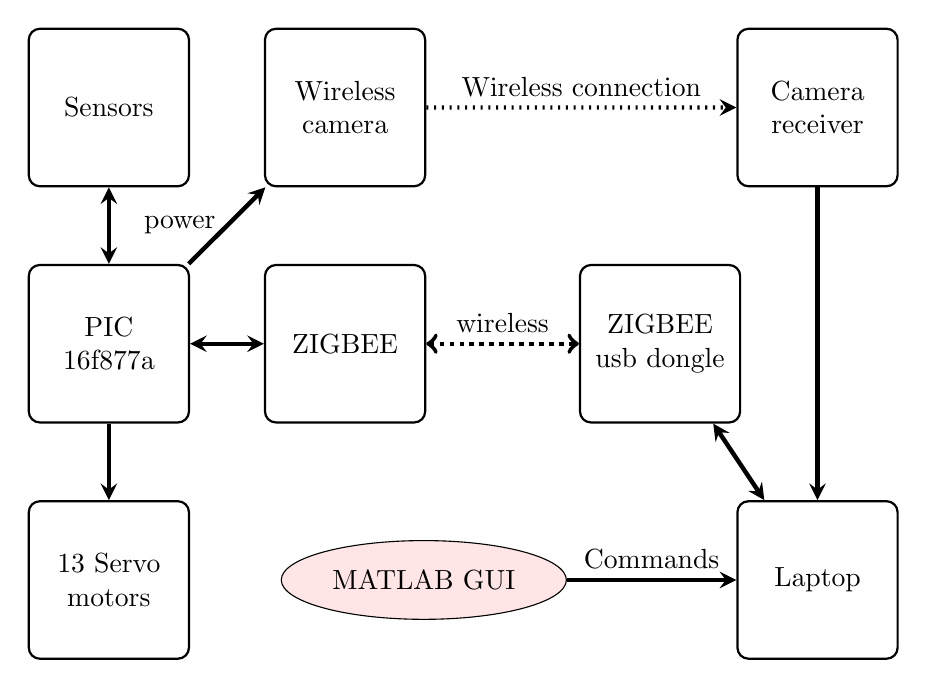
\begin{tikzpicture}[node distance=2cm]

\node(laptop)[box] at (0,0) {Laptop};
\node(zigbeeusb)[box,above  of=laptop,yshift=+1cm,xshift=-2cm] {ZIGBEE usb dongle}; 
\node(zigbee)[box,left of=zigbeeusb,xshift=-2cm] {ZIGBEE};
\node(pic)[box,left of=zigbee,xshift=-1cm] {PIC 16f877a};
\node(receiver)[box,above of=laptop,yshift=4cm]{Camera receiver};
\node(servo)[box,above of=pic,yshift=-5cm] {13 Servo motors};
\node(sensor)[box,above of=pic,yshift=+1cm] {Sensors};
\node(camera)[box,above of=zigbee,yshift=1cm]{Wireless camera};

\node(gui)[gui,left of=laptop,xshift=-3cm]{MATLAB GUI};


\draw [<->,>=stealth,ultra thick] (laptop) --(zigbeeusb);

\draw [<->,>=stealth,ultra thick](zigbee)--(pic);
\draw [<->,ultra thick,dotted](zigbee)--node [anchor=south]{wireless}(zigbeeusb);
\draw [->,>=stealth,ultra thick] (pic) --(servo);
\draw [<->,>=stealth,ultra thick] (pic) --(sensor);
\draw [->,>=stealth,ultra thick] (gui) --node [anchor=south]{Commands}(laptop);

\draw [arrow,ultra thick] (pic) -- node [anchor=east] {power}(camera);

\draw [arrow,dotted,ultra thick] (camera)-- node[anchor=south]{Wireless connection}(receiver);

\draw [arrow,ultra thick] (receiver)--(laptop);
\end{tikzpicture}
\caption{System structure}
\label{fig33}
\end{center}
\end{figure}
 %block diagram ends

\section{Wlaking pattern}
The Hexapod robot in this project uses the famous tripod gait for locomotion.\\
In the following drawings a dark circle means the foot is firmly planted on the ground and is supporting the weight of the robot. A light circle means the foot is not supporting any weight and is movable.\\
This gait is a fast gait for the hexapod; it completes a cycle in two beats. In this gait the robot lift three legs simultaneously while leaving three legs on the ground, which keeps the robot stable.\\
This is called a tripod gait, because a tripod positioning of legs always supports the weight of the walker\\
\begin{figure}[h!]
\centering
\includegraphics[scale=1]{tripodgait}
\caption{PWM pattern for each leg}
\label{fig34}
\end{figure}
\subsection{Walking forward}
We start in the rest position (see Fig. ~\ref{35}\ ). As before, each circle represents a foot, and the dark circles
show the weightbearing feet. Notice in the rest position, the center legs do not support any weight. These
center legs are made to be 1/8 in shorter than the front and back legs.\\
In position A the center legs are rotated CW by about 25 from center position. This causes the robot to tilt to the right. The weight distribution is now on the front and back right legs and the center left leg.
This is the standard tripod position as described earlier. Since there is no weight on the front and back left
legs, they are free to move forward as shown in the B position of Fig. ~\ref{35}\ \\
In the C position the center legs are rotated CCW by about 25 from center position. This causes the
robot to tilt to the left. The weight distribution is now on the front and back left legs and the center right
leg. Since there is no weight on the front and back right legs, they are free to move forward, as shown in the
D position\\
In position E the center legs are rotated back to their center position. The robot is not in a tilted position
so its weight is distributed on the front and back legs. In the F position, the front and back legs are moved
backward simultaneously, causing the robot to move forward. The walking cycle can then repeat.
\begin{figure}[h!]
\centering
\includegraphics[width=\textwidth]{fig103}
\caption{Forward gait for hexapod robot}
\label{35}
\end{figure}
\FloatBarrier
\subsection{Moving backward}
We start in the rest position (see Fig. ~\ref{fig36}\ ), as before. In position A the center legs are rotated CW by
about 25 from center position. The robot tilts to the right. The weight distribution is now on the front and
back right legs and the center left leg. Since there is no weight on the front and back left legs, they are free
to move backward, as shown in the B position of Fig. ~\ref{fig36}\ \\
In the C position the center legs are rotated CCW by about 25 from center position. The robot tilts
to the left. Since there is no weight on the front and back right legs, they are free to move backward, as
shown in the D position.\\
In position E the center legs are rotated back to their center position. The robot is not in a tilted position,
so its weight is distributed on the front and back legs. In the F position, the front and back legs are moved
forward simultaneously, causing the robot to move backward. The walking cycle can then repeat\\
\begin{figure}[h!]
\centering
\includegraphics[width=\textwidth]{fig104}
\caption{Backward gait for hexapod robot}
\label{fig36}
\end{figure}
\FloatBarrier
\subsection{Turning left}
The leg motion sequence to turn left is shown in Fig. ~\ref{fig37}. In position A the center legs are rotated CW by
about 25 from center position. The robot tilts to the right. The weight distribution is now on the front and
back right legs and the center left leg. Since there is no weight on the front and back left legs, they are free
to move forward, as shown in Fig. ~\ref{fig37}\ \\
In the B position, the center legs are rotated CCW by about 25 from center position. The robot tilts to the
left. Since there is no weight on the front and back right legs, they are free to move backward, as shown in the
C position\\
In position D, the center legs are rotated back to their center position. The robot is not in a tilted position, so its weight is distributed on the front and back legs. In position, the left legs moved backward while
the right legs moved forward, simultaneously causing the robot to turn left. It typically takes three turning
cycles to turn the robot 90.\\
\begin{figure}[h!]
\centering
\includegraphics[width=\textwidth]{fig105}
\caption{Turning-left}
\label{fig37}
\end{figure}
\FloatBarrier
\subsection{Turning right}
Turning right follows the same sequence as turning left, with the leg positions reversed.\\
\section{Servo control}
The motion of the robot is controlled by controlling the servos attached to each leg in a specific pattern.
\subsection*{Introduction}
Servo motors are electro-mechanical devices which provide good torque . If you open a servo motor you will
see a simple DC motor connected to a potentiometer and as motor rotates output value of potentiometer
also changes . Now a servo motor has three wires rst one for voltage ,second for data and third for ground
. Generally value for voltage is 5V but always check your motor ratings. Now see servo motor expects a
pulse every 20ms and width of the pulse varies from 1ms to 2ms. 1ms for maximum rotation in one direction
lets say -90 and 2ms for +90\\
There are many methods for moving servo motors i.e generating the required pulses we used timer0 for generating an interrupt every 20ms and then send
a pulse using delay function.\\
The 12 servo motors are controlled by the pwm signals generated by the PIC microcontroller.
The  code for motor control is written in C language using MPLAB with HI-TECH C compiler. 

In the circuit, PIC16F877A is running on external crystal of 20MHz value. RA0 pin is toggled every time timer0 expires and executes it's ISR(Interrupt Service Routine) code.\\
\subsection*{PWM generation}
The code used to initialize timer0 is shown below.\\

\begin{lstlisting}[caption=Timer0 Initialisation]
void InitTimer0(void)
{
//Timer0 is 8 bit timer, select TOCS and PSA to be zero
OPTION_REG = 0xC0;	//Make prescalar 1:2

T0IE = 1;			// Enable Timer0 interrupt
GIE = 1;			// Enable global interrupts
}
\end{lstlisting}

In this function, OPTION\_ REG is initialized to make timer0 prescalar to be 1:2. Timer0 is an 8bit timer, so it expires after reaching a value of 255. When timer0 prescalar is made 1:2 then it means that timer0 value will increment after every two clock cycles. T0IE bit enables timer0 interrupts and GIE bit enables global interrupts.

Timer0 interrupt service routine code is shown below.\\
\begin{lstlisting}[caption= Timer0 Interrupt service routine,label=fig32]
void interrupt ISR(void)
{
	if(T0IF)	//If Timer0 interrupt is set
	{
		RA0=~RA0;	// Toggle RA0 pin
		T0IF=0 ; 	// Clear the interrupt
	}
}
\end{lstlisting}
Whenever timer0 expires, then an interrupt is generated which executes the function shown above in the Figure ~\ref{fig32}. In this function, RA0 pin is toggled every time and timer0 interrupt flag is cleared. This means that whenever RA0 pin toggles then timer0 interrupt has occurred.
In the main function, firstly TRISA0 is made zero to make RA0 pin an output pin, also RA0 pin is made zero. After that, InitTimer0() function is called which initializes timer0. Rest of the work is done in timer0 interrupt service routine as explained below. Every time timer0 expires RA0 pin is toggled.\\
The following section shows how to  interrupt subroutine to control the duty cycle of each PWM channel. In the interrupt subroutine, an interrupt counter is incremented once for every interrupt happened and can be used for the duration calculation of each pin’s high level output. Assuming the duty cycle of each PWM channel is calculated in the beginning of every interrupt cycle. Comparing the preset duty cycle of each channel and the time of duration, the corresponding pin will be reset as zero if the equal condition is satisfied. Therefore, the duty cycle of each channel is under control. Also, based on the precise time base, a preset interrupt mcounter bound is used to tune the PWM period. Once the upper bound of interrupt counter is achieved, the interrupt counter will be reset as zero and all the pins’ outputs are reset at high level.\\

Program ~\ref{ISR}\ is the partial code of interrupt subroutine to illustrate above operation. In program 1, interrupt\_ count×time\_ base denotes the duration time of each PWM cycle. Comparing the duration time with the preset duty cycle of each channel set\_ PWM\_ duty[i], if the equal condition is satisfied, the corresponding IO pin will be reset as LOW. The final if instruction is used to tune the PWM period (frequency). Once the equal condition is satisfied, the interrupt\_ count will be reset as 0 and all the PWM IO pins reset as LOW. The PWM period is count\_ upper\_ bound × time\_ base. 
\begin{lstlisting}[caption= ISR, label= ISR]
void interrupt_h_function(void) //interrupt function
{
.....;
.....;
interrupt_count=interrupt_count+1;//interrupt_count
//incremented
if(interrupt_ count ==set_PWM_duty[0])//Is the duty cycle
//of channel 1 achieved?
PWM_1=0;//reset the corresponding IO pin 1 as /LOW
if(interrupt_ count ==set_PWM_duty[1]) //Is the duty cycle
//of channel 2 achieved?
PWM_2=0;//reset the corresponding IO pin 2 as //LOW
if(interrupt_ count ==set_PWM_duty[2]) //Is the duty cycle
//of channel 3 achieved?
PWM_3=0;//reset the corresponding IO pin 3 as LOW
.....;
if(interrupt_count==set_PWM_duty[n]) //Is the duty cycle
//of channel n achieved?
PWM_n=0;//reset the corresponding IO pin 3 as LOW
if(interrupt_count==count_upper_bound) //Does the
//interrupt_ count upper bound achieved?
{ interrupt_count=0;//reset the interrupt_count value
PORTD=0XFF; //reset the corresponding IO pins
PORTJ=0XFF;
PORTF=0XFF;
PORTB=0XFF;
}
.....;
.....;
}
\end{lstlisting}
\subsection{Flowcharts}
The flow charts for the main program (Fig. ~\ref{flw5a}) and the Interrupt Service Routine (Fig. ~\ref{flw5b}) are given below


% Main Program
\begin{figure}
\begin{center}
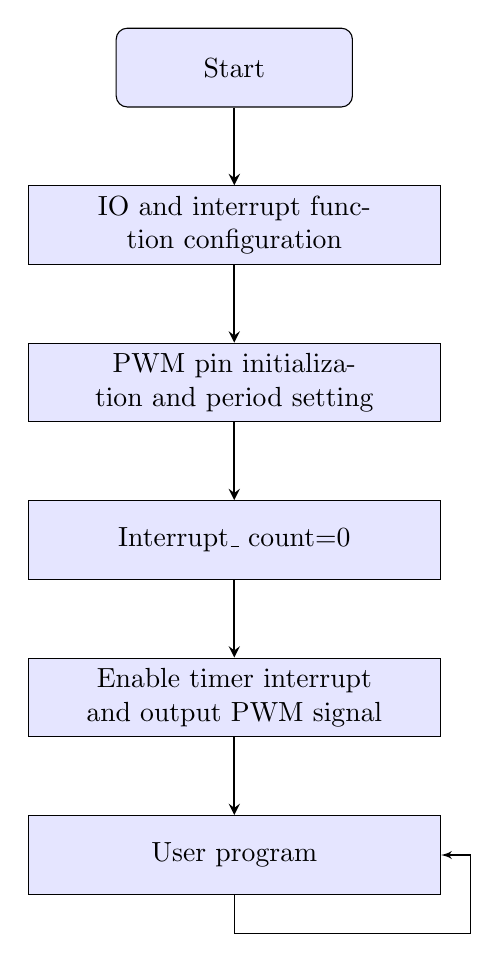
\begin{tikzpicture}[node distance=2cm]


\node (start) [startstop] {Start};
%\node (in1) [io, below of=start] {Input};
\node (pro1) [process, below of=start] {IO and interrupt function configuration};
%\node (dec1) [decision, below of=pro1, yshift=-0.5cm] {Decision 1};
\node (pro2) [process, below of=pro1] {PWM pin initialization and period setting};
\node (pro3) [process, below of=pro2] {Interrupt\_ count=0};
\node (pro4) [process, below of=pro3] {Enable timer interrupt and output PWM signal};
\node (pro5) [process, below of=pro4] {User program};

\draw [arrow] (start) -- (pro1);
\draw [arrow] (pro1) -- (pro2);
\draw [arrow] (pro2) -- (pro3);
\draw [arrow] (pro3) -- (pro4);
\draw [arrow] (pro4) -- (pro5);
%\draw [arrow] (pro5) |- ($(arrow.south east) + (0.5,-0.5)$) |- (pro4);  
\path[line] (pro5) |- +(3,-1) |- (pro5.east);  
\end{tikzpicture}
\end{center}
\caption{Main Program Flowchart}
\label{flw5a}
\end{figure}

\begin{figure}
\begin{center}
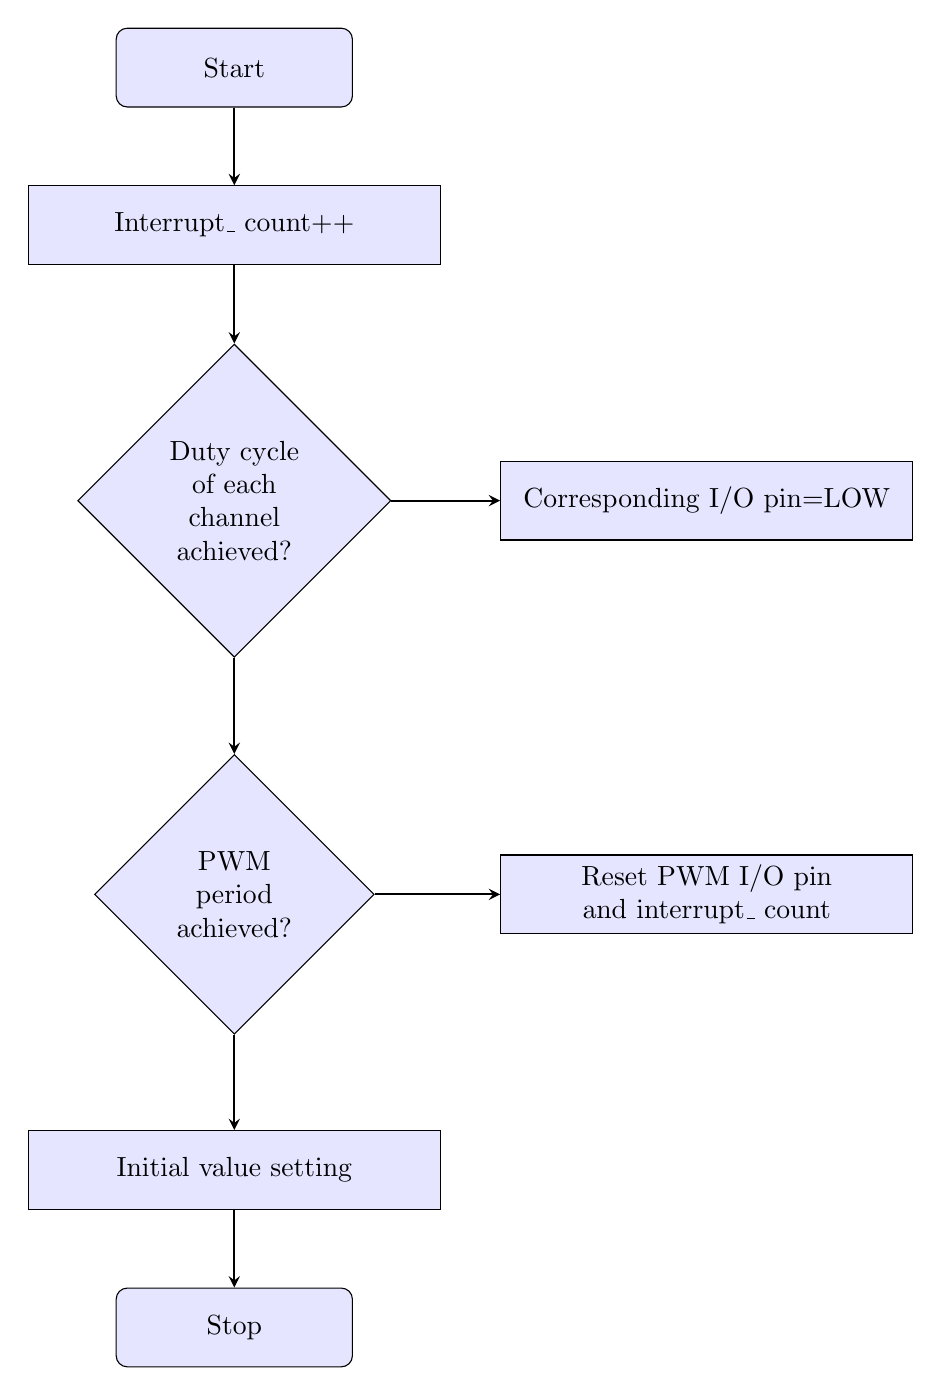
\begin{tikzpicture}[node distance=2cm]
\node(start)[startstop]{Start};
\node(pro1)[process,below of=start]{Interrupt\_ count++};
\node(dec1)[decision,below of=pro1,yshift=-1.5cm]{Duty cycle of each channel achieved?};
\node(dec2)[decision,below of=dec1,yshift=-3.0cm]{PWM period achieved?};
\node(pro2)[process,right of=dec1,xshift=+4.0cm]{Corresponding I/O pin=LOW};
\node(pro3)[process,right of=dec2,xshift=+4.0cm]{Reset PWM I/O pin and interrupt\_ count};
\node(pro4)[process,below of=dec2,yshift=-1.5cm]{Initial value setting};
\node(stop)[startstop,below of=pro4]{Stop};

\draw[arrow] (start) -- (pro1);
\draw[arrow] (pro1) -- (dec1);
\draw[arrow] (dec1) -- (dec2);
\draw[arrow] (dec2) -- (pro4);
\draw[arrow] (pro4) -- (stop);
\draw[arrow] (dec1) -- (pro2);
\draw[arrow] (dec2) -- (pro3);


\end{tikzpicture}
\end{center}
\caption{Interrupt subroutine flow chart}
\label{flw5b}
\end{figure}
%Flowchart ends
\section{GUI creation using Matlab}
The guided user interface for the control of the robot was created using Matlab GUI tool.
The GUI code used for the project is included in the annexures
The final GUI is shown in figure ~\ref{fig38}
\begin{figure}[h!]
\centering
\includegraphics[width=\textwidth]{gui001}
\caption{GUI created using Matlab}
\label{fig38}
\end{figure}
\FloatBarrier

The buttons used are:
\begin{itemize}
\item \emph{COM PORT} : To set up zigbee with pc ports
\item \emph{Image Data} : To obtain output of weed detection
\item CONTROLS
\begin{itemize}
\item \emph{Forward} : Forward command
\item \emph{Backward} : Backward command
\item \emph{Left}	: Left movement
\item \emph{Right}	: Right movement
\item \emph{Stop}	:Stop motion
\end{itemize}
\item \emph{Sensor Data} : To display the sensor values
\item \emph{STOP} : To stop reading sensor values
\end{itemize}
\section{Weed detection using Matlab}
Figure ~\ref{fig39} shows obtained output for a sample input\\

\begin{figure}[h!]
\centering

\begin{subfigure}{0.5\textwidth}
	\includegraphics[width=\textwidth]{image.jpg}
	\caption{Sample Input}
	\label{fig39a}
\end{subfigure}
\begin{subfigure}{0.5\textwidth}
	\includegraphics[width=\textwidth]{imagedata}
	\caption{Obtained output}
	\label{fig39b}
\end{subfigure}
\caption{Weed Detection using Matlab}
\label{fig39}
\end{figure}
\FloatBarrier
In the whole image the red plants are supposed to be the crops and the green plants in between them are supposed to be weeds.
As shown in figure ~\ref{fig39b} the matlab code succesfully identified the weeds.
The code is based on simple colour detection principle. In the future we are planning to expand the project and making it capable of detecting more types of weeds using leaf pattern detection and Neural networks.\\
\subsection*{Steps involved}
\begin{enumerate}
\item The intensity of the RGB values are increased using the function imadjust
\item	The green part of the image is considered as foreground. Then the imsubtract operation is done between the 'G' dimension values and the grey scale image
\item	To suppress the background median filtering is done
\item	The resulting image is converted into black and white. Thus the green pixels are now seen as white pixels and the rest of the background is changed to black
\item	Next the image is divided into three segments and each segment is checked for white pixels
\item	If the number of white pixels is beyond a fixed threshold then the robot decides that there are weeds in the area and destroys the weeds by drilling the roots with a dc motor. Otherwise if the value is less than the threshold then the robot moves on
\end{enumerate}


\chapter{CONCLUSION AND FUTURE SCOPE}
The goal of this project was to create a Hexapod robot for Agricultural applications. The long term goal was to make it intelligent to fully take over all the operations in a farm. The main target operations included:\\
\begin{itemize}
\item Tills the soil within a few centimeters of the seed
\item	Plants Seeds at precise intervals and records the position of planting
\item	Scouts the field for weed detection
\item	Weeding : Applies weedicide at only areas where there is high concentration of weeds
\end{itemize}
We were able to build a satisfactory prototype of the hexapod robot with six legs each controlled by two servo motors. The hexapod Tripod gait algorithm was also succesfully implemented.
The final robot is found to be highly manoeuvrable and versatile and it could traverse even rough terrain easily.\\
Coming to the Agricultural applications; we successfully implemented the following systems in our prototype:
\begin{itemize}
\item Weed detection capability was examined using Matlab colour detection principles
\item Obstacle avoidance algorithms were successfully implemented. This could allow the robot to navigate without human interference guided by the boundaries of the farm.
\item Sensors on-board worked perfectly showing the possibilities of remote data collection 
\end{itemize}
Building such robot provide an infinite possibilities of applications such as SAR (Search and Rescue) ,
RFID(Radio-frequency identification) tracker, face detection, fire detector, mine detector and many other military applications. But first we are planning to add micro-sprayers, a mechanical hand and other add-ons to improve the capabilities of the robot in the field of Agriculture.\\
Some of our other more ambitious plans are listed below:
\begin{enumerate}
\item	Each leg of the hexapod can be fitted with pressure sensors . The input from these pressure sensors can be used to implement algorithms than change the step lengths and the walking patterns (gaits ) of the hexapod according to the external environment
\item It is possible to extract length measurements of real life objects from the captured image using Digital Image Processing .
The collected data can be used by the hexapod to avoid too deep holes or very high obstacles
\item	In Agriculture; productivity can be improved by using Swarm Robotics. The hexapod in this project has the ability to perform sowing seeds, removing weeds and harvesting more efficiently as discussed in this paper. 
A swarm of hexapods can thus replace the farmers and perform almost all the farming procedures. 
\item	Artificial Intelligence algorithms can be used to improve the efficiency of image processing algorithms
\item	If the servo motors are replaced by pneumatic pistons or electronic muscle fibres then the robot can support more weight
\item If it’s possible to design a life sized Hexapod then it will be a more stable means of locomotion for the physically challenged.
It will allow them to climb steps and move through rocky terrain without the need of getting down from the machine

\end{enumerate} 

\renewcommand{\bibname}{REFERENCES}
\begin{thebibliography}{9}

\bibitem{lamport94}
  Chin-Pao Hung,Wei-Ging Liu,Hong-Jhe Su,Jia-Wei Chen and Bo-Ming Chiu, 
  \emph{PIC-Based Multi-Channel PWM Signal Generation Method and Application to Motion Control of Six Feet Robot Toy}'
  International Journal Of Circuits, Systems and Signal Processing,
  Issue 2,Volume 3,
  2009.

\bibitem{simulating}
Ing.R.Woering,\emph{Simulating the first steps of a walking hexapod robot},Technische Universiteit Eindhoven,Department Mechanical Engineering,Control Systems Technology Group,Eindhoven,Eindhoven,January,2011.

\bibitem{Pedersen}
Pedersen S.M,Fountas S and Blackmore S,
\emph{Agricultural Robots-Applications and Economic Prespectives},University of Copenhagen,Institute of Food and Resource Economics, University of Thessaly,Denmark,Greece.

\bibitem{Jordanian University}
Tareq Mamkegh,Ahmad Hindash and Mohammad Al-Jabari,\emph{Hexapod Robot-Robot Design,model and control},German Jordanian University,May 2011.

\bibitem{ArduinoCookbook}
Michael Margolis,
\emph{Arduino Cookbook},
O'Reilly,
Second Edition,
December 2011,
ISBN 13: 978-93-5023-612-3

\bibitem{Web}
\emph{Arduino Examples},\ \hyperref[tosee]{\color{red}\url{http://arduino.cc/en/Tutorial/HomePage}}

%\url{\color{blue}}}
\end{thebibliography}

%Appendix starts
\begin{appendices}

\chapter{16f877a Datasheet}
\includepdf[pages={3-5,8,10-11,13,21-22,49-51,97-100
,101-106,113-115,116-118},scale=0.8]{PIC16F877A}

\chapter{Source Code - PIC 16f877a}
%Code block starts

\begin{lstlisting}
// Hexapod.C
#include<pic.h>
int Timer_count=0,i;
char  array[6];
char  array_value,k,angle;
//char j;
void timer0_int(void);
void usart_init(void);
int convert_angle(char angle);
void servo_init(void);
void servo_246_init(void);
void servo_135_init(void);
void angle_init(void);

void forward();
void Backward();
void Left(void);
void Right(void);
void Clockwise();
void Anti_Clockwise();
void start(void);
void Stop();
void display(char );
 void MSdelay(unsigned int val);
char RECDATA;
int adcvalue=0;
int Temp_value=0;
int Humd_value=0;
int LDR_value=0;
int IR_value=0;
int mems_value=0;
int obstacle_threshold=300;
int  ADC_read(char channel );
void obstacles_avoidance(void);

/****************OUTER SERVOS***************/
#define servo_motor1  RD2
#define servo_motor2  RD3
#define servo_motor3  RD4
#define servo_motor4  RD5
#define servo_motor5  RD6
#define servo_motor6  RB7
/***************INNER SERVOS***************/
#define servo_motor11   RB2
#define servo_motor22  RB3
#define servo_motor33  RB4
#define servo_motor44  RB5
#define servo_motor55  RB6
#define servo_motor66  RB1

#define Head_servo_motor  RD7;
char Head_servo_motor_value;

char servo_motor1_value;
char servo_motor2_value;
char servo_motor3_value;
char servo_motor4_value;
char servo_motor5_value;
char servo_motor6_value;

char servo_motor11_value;
char servo_motor22_value;
char servo_motor33_value;
char servo_motor44_value;
char servo_motor55_value;
char servo_motor66_value;

char servo_motor1_angle;
char servo_motor2_angle;
char servo_motor3_angle;
char servo_motor4_angle;
char servo_motor5_angle;
char servo_motor6_angle;

char servo_motor11_angle;
char servo_motor22_angle;
char servo_motor33_angle;
char servo_motor44_angle;
char servo_motor55_angle;
char servo_motor66_angle;
char Head_servo_motor_angle;
void main()
{
	TRISD = 0X00;

	TRISB = 0X00;
		TRISA = 0Xff;
	timer0_int();
	usart_init();
	angle_init();
	servo_init();
	ADCON1=0X82;
	MSdelay(1000);
	//start();
	//Clockwise();//
	//forward();
	//Backward();
	//Left();
while (1)
{
if(RECDATA=='F'){forward();obstacles_avoidance();}
if(RECDATA=='B'){Backward();}
if(RECDATA=='L'){Left();}
if(RECDATA=='R'){Right();}

if(RECDATA=='C'){Clockwise();}
if(RECDATA=='A'){Anti_Clockwise();}

if(RECDATA=='S'){Stop();}

	 
	MSdelay(100);
	 Temp_value=ADC_read( 0X81);  
	 Temp_value=(int)(Temp_value*.4);
	 LDR_value=ADC_read( 0X89);  
	 Humd_value=ADC_read( 0X91); 
	 Humd_value=(int)(Humd_value/6.67);
	
	mems_value=ADC_read( 0XA1);

%	TXREG='#';while(TRMT!=1);
	TXREG='$';while(TRMT!=1);
	display(Temp_value);

	TXREG='$';while(TRMT!=1);
	display(LDR_value);

	TXREG='$';while(TRMT!=1);
	display(Humd_value);
	TXREG='$';while(TRMT!=1);
	display(mems_value);
	TXREG='$';while(TRMT!=1);
	TXREG='*';while(TRMT!=1);
	MSdelay(1000);
}
}
void interrupt ad()
{
if(T0IF==1)
{
T0IF=0;
Timer_count++;
if(Timer_count<125){
TMR0 	= 213;           //Timer value for 20micro second
}
if(Timer_count==servo_motor1_value)
	servo_motor1=0;
if(Timer_count==servo_motor2_value)
	servo_motor2=0;
if(Timer_count==servo_motor3_value)
	servo_motor3=0;
if(Timer_count==servo_motor4_value)
	servo_motor4=0;
if(Timer_count==servo_motor5_value)
	servo_motor5=0;
if(Timer_count==servo_motor6_value)
	servo_motor6=0;
if(Timer_count==servo_motor11_value)
	servo_motor11=0;
if(Timer_count==servo_motor22_value)
	servo_motor22=0;
if(Timer_count==servo_motor33_value)
	servo_motor33=0;
if(Timer_count==servo_motor44_value)
	servo_motor44=0;
if(Timer_count==servo_motor55_value)
	servo_motor55=0;
if(Timer_count==servo_motor66_value)
	servo_motor66=0;
if(Timer_count==Head_servo_motor_value)
//	Head_servo_motor=0;

if(Timer_count>=125)
{
 	PS2=1;
	PS1=1;
	PS0=0;
	TMR0=122;
}
if( Timer_count == 130 )
	{ 
	PORTD=0XFF;
	PORTB=0XFF;
	PS2=0;
	PS1=0;
	PS0=0;
    	TMR0=213;
    	Timer_count = 0;
	}
}
if(RCIF==1)
{
RCIF=0;
RECDATA=RCREG;


}
}
void timer0_int()
{
	PSA 	= 0;
	PS2 	= 0;
	PS1 		= 0;
	PS0 	= 0;
	GIE 	= 1;
	PEIE 	= 1;
	T0IE 	= 1;
	TMR0 	= 215;
	T0CS 	= 0;
}
void usart_init()
{
	TXEN	=1;
	BRGH	=1;
	SPBRG	=10;
	SYNC	=0;
	SPEN	=1;
	CREN	=1;
	GIE		=1;
	PEIE	=1;
	RCIE	=1;
	TRISC	=0X80;
}
void display(char angle )
{
	char  array_value1;
	array_value1=angle;
	for(i=1;i<=3;i++)
	{
	array[i]=array_value1%10;
	array_value1=array_value1/10;
	}
	for(i=3;i>=1;i--)
	{
	TXREG=array[i]+'0';
	while(TRMT!=1);
	}
	TXREG=0x0D;while(TRMT!=1);
	TXREG=0x0A;while(TRMT!=1);
}	
void servo_init()
{

	 servo_motor1_angle=29;
	 servo_motor2_angle=28;
	 servo_motor3_angle=25;
	 servo_motor4_angle=28;
	 servo_motor5_angle=26;
	 servo_motor6_angle=30;
	 servo_motor11_angle=26;
	 servo_motor22_angle=18;
	 servo_motor33_angle=25;
	 servo_motor44_angle=26;
	 servo_motor55_angle=20;
 	 servo_motor66_angle=30;	


	 servo_motor1_value = convert_angle( servo_motor1_angle);
	 servo_motor2_value = convert_angle( servo_motor2_angle);
	 servo_motor3_value = convert_angle( servo_motor3_angle);
	 servo_motor4_value = convert_angle( servo_motor4_angle);
	 servo_motor5_value = convert_angle( servo_motor5_angle);
	 servo_motor6_value = convert_angle( servo_motor6_angle);
	
	 servo_motor11_value = convert_angle ( servo_motor11_angle);
	 servo_motor22_value = convert_angle( servo_motor22_angle);
	 servo_motor33_value = convert_angle( servo_motor33_angle);
	 servo_motor44_value = convert_angle( servo_motor44_angle);
	 servo_motor55_value = convert_angle( servo_motor55_angle);
 	 servo_motor66_value = convert_angle( servo_motor66_angle);
}
void angle_init()
{
	 servo_motor1_angle=29;
	 servo_motor2_angle=28;
	 servo_motor3_angle=26;
	 servo_motor4_angle=28;
	 servo_motor5_angle=27;
	 servo_motor6_angle=30;
	 servo_motor11_angle=26;
	 servo_motor22_angle=18;
	 servo_motor33_angle=25;
	 servo_motor44_angle=26;
	 servo_motor55_angle=20;
 	 servo_motor66_angle=29;
	
}

void servo_135_init()
{
//	 servo_motor1_angle=29;
//	 servo_motor3_angle=25;
//	 servo_motor5_angle=27;
//	 servo_motor11_angle=26;
//	 servo_motor33_angle=25;
//	 servo_motor55_angle=20;

	 servo_motor1_angle=29;
	 servo_motor3_angle=25;
	 servo_motor5_angle=27;
	 servo_motor11_angle=26;
	 servo_motor33_angle=25;
	 servo_motor55_angle=20;

	 servo_motor1_value = convert_angle( servo_motor1_angle);
	 servo_motor3_value = convert_angle( servo_motor3_angle);
	 servo_motor5_value = convert_angle( servo_motor5_angle);
	 servo_motor11_value = convert_angle ( servo_motor11_angle);
	 servo_motor33_value = convert_angle( servo_motor33_angle);
	 servo_motor55_value = convert_angle( servo_motor55_angle);
}
void servo_246_init()
{
//	 servo_motor2_angle=28;
//	 servo_motor4_angle=28;
//	 servo_motor6_angle=30;
//	 servo_motor22_angle=18;
//	 servo_motor44_angle=26;
// 	 servo_motor66_angle=30;


	 servo_motor2_angle=28;
	 servo_motor4_angle=28;
	 servo_motor6_angle=30;
	 servo_motor22_angle=18;
	 servo_motor44_angle=26;
 	 servo_motor66_angle=29;
	 servo_motor2_value = convert_angle( servo_motor2_angle);
	 servo_motor4_value = convert_angle( servo_motor4_angle);
	 servo_motor6_value = convert_angle( servo_motor6_angle);
	 servo_motor22_value = convert_angle( servo_motor22_angle);
	 servo_motor44_value = convert_angle( servo_motor44_angle);
 	 servo_motor66_value = convert_angle( servo_motor66_angle);
}
/***************/
/*
												Forward movemenht of Robort
*/
/***************/
void forward()
{

for (k=0;k<15;k++)
{
	servo_motor1_value=convert_angle(servo_motor1_angle++);
	servo_motor3_value=convert_angle(servo_motor3_angle++);        
	servo_motor5_value=convert_angle(servo_motor5_angle++);
	MSdelay(35);
}

for (k=0;k<15;k++)
{
	
	servo_motor11_value = convert_angle(servo_motor11_angle++);
	servo_motor33_value=convert_angle(servo_motor33_angle--);
	servo_motor55_value=convert_angle(servo_motor55_angle--);
	MSdelay(35);
}

for (k=0;k<15;k++)
{
	
	servo_motor1_value=convert_angle(servo_motor1_angle--);
	servo_motor3_value=convert_angle(servo_motor3_angle--);
	servo_motor5_value=convert_angle(servo_motor5_angle--);
	MSdelay(35);
}

///***************/
for (k=0;k<15;k++)
{

	servo_motor2_value=convert_angle(servo_motor2_angle++);
	servo_motor4_value=convert_angle(servo_motor4_angle++);
	servo_motor6_value=convert_angle(servo_motor6_angle++);	
	MSdelay(35);
}

for (k=0;k<15;k++)
{
	MSdelay(35);	
	servo_motor11_value=convert_angle(servo_motor11_angle--);
	servo_motor33_value=convert_angle(servo_motor33_angle++);
	servo_motor55_value=convert_angle(servo_motor55_angle++);
}

servo_135_init();


for (k=0;k<15;k++)
{
	MSdelay(35);	
	servo_motor22_value=convert_angle(servo_motor22_angle++);
	servo_motor44_value=convert_angle(servo_motor44_angle--);
	servo_motor66_value=convert_angle(servo_motor66_angle++);
}
for (k=0;k<15;k++)
{
	
	servo_motor2_value=convert_angle(servo_motor2_angle--);
	servo_motor4_value=convert_angle(servo_motor4_angle--);
	servo_motor6_value=convert_angle(servo_motor6_angle--);	
	MSdelay(35);
}


for (k=0;k<15;k++)
{
	MSdelay(35);
	servo_motor1_value=convert_angle(servo_motor1_angle++);
	servo_motor3_value=convert_angle(servo_motor3_angle++);
	servo_motor5_value=convert_angle(servo_motor5_angle++);
}
for (k=0;k<15;k++)
{
	MSdelay(35);
	servo_motor22_value=convert_angle(servo_motor22_angle--);
	servo_motor44_value=convert_angle(servo_motor44_angle++);
	servo_motor66_value=convert_angle(servo_motor66_angle--);
	
}
servo_246_init();


}
/***************/
/*
									Backward movemenht of Robort
*/
/***************/
void Backward()
{

//for (k=0;k<15;k++)
//{
//	servo_motor1_value=convert_angle(servo_motor1_angle++);
//	servo_motor3_value=convert_angle(servo_motor3_angle++);         /*        motot1,3,5 raise upward direction          */
//	servo_motor5_value=convert_angle(servo_motor5_angle++);
//MSdelay(35);
//}
for (k=0;k<15;k++)
{
	
	servo_motor11_value = convert_angle(servo_motor11_angle--);
	servo_motor33_value=convert_angle(servo_motor33_angle--);
	servo_motor55_value=convert_angle(servo_motor55_angle++);
MSdelay(35);
}

for (k=0;k<15;k++)
{
	
	servo_motor1_value=convert_angle(servo_motor1_angle--);
	servo_motor3_value=convert_angle(servo_motor3_angle--);
	servo_motor5_value=convert_angle(servo_motor5_angle--);
MSdelay(35);
}

/***************/
for (k=0;k<15;k++)
{

	servo_motor2_value=convert_angle(servo_motor2_angle++);
	servo_motor4_value=convert_angle(servo_motor4_angle++);
	servo_motor6_value=convert_angle(servo_motor6_angle++);	
MSdelay(35);
}
//
for (k=0;k<15;k++)
{
	MSdelay(35);	
	servo_motor11_value=convert_angle(servo_motor11_angle++);
	servo_motor33_value=convert_angle(servo_motor33_angle++);
	servo_motor55_value=convert_angle(servo_motor55_angle--);
}

servo_135_init();


for (k=0;k<15;k++)
{
	MSdelay(35);	
	servo_motor22_value=convert_angle(servo_motor22_angle--);
	servo_motor44_value=convert_angle(servo_motor44_angle++);
	servo_motor66_value=convert_angle(servo_motor66_angle++);
}
for (k=0;k<15;k++)
{
	
	servo_motor2_value=convert_angle(servo_motor2_angle--);
	servo_motor4_value=convert_angle(servo_motor4_angle--);
	servo_motor6_value=convert_angle(servo_motor6_angle--);	
MSdelay(35);
}


for (k=0;k<15;k++)
{
	MSdelay(35);
	servo_motor1_value=convert_angle(servo_motor1_angle++);
	servo_motor3_value=convert_angle(servo_motor3_angle++);
	servo_motor5_value=convert_angle(servo_motor5_angle++);
}
for (k=0;k<15;k++)
{
	MSdelay(35);
	servo_motor22_value=convert_angle(servo_motor22_angle++);
	servo_motor44_value=convert_angle(servo_motor44_angle--);
	servo_motor66_value=convert_angle(servo_motor66_angle--);	
}
servo_246_init();
}

/***************/
/*						left movements    										   */
/***************/
void Left()
{
/*for (k=0;k<15;k++)
{
	servo_motor1_value=convert_angle(servo_motor1_angle++);
	servo_motor3_value=convert_angle(servo_motor3_angle++);        
	servo_motor5_value=convert_angle(servo_motor5_angle++);
	MSdelay(35);
}*/ 
//start();
for (k=0;k<15;k++)
{
	
	servo_motor11_value = convert_angle(servo_motor11_angle--);
	servo_motor33_value=convert_angle(servo_motor33_angle--);
	servo_motor55_value=convert_angle(servo_motor55_angle++);
	MSdelay(35);
}


for (k=0;k<15;k++)
{
	
	servo_motor1_value=convert_angle(servo_motor1_angle--);
	servo_motor3_value=convert_angle(servo_motor3_angle--);
	servo_motor5_value=convert_angle(servo_motor5_angle--);
	MSdelay(35);
}

///***************/
for (k=0;k<15;k++)
{

	servo_motor2_value=convert_angle(servo_motor2_angle++);
	servo_motor4_value=convert_angle(servo_motor4_angle++);
	servo_motor6_value=convert_angle(servo_motor6_angle++);	
	MSdelay(35);
}

for (k=0;k<15;k++)
{
	
	servo_motor11_value = convert_angle(servo_motor11_angle++);
	servo_motor33_value=convert_angle(servo_motor33_angle++);
	servo_motor55_value=convert_angle(servo_motor55_angle--);
	MSdelay(35);
}
servo_135_init();


for (k=0;k<15;k++)
{
	MSdelay(35);	
	servo_motor22_value=convert_angle(servo_motor22_angle--);
	servo_motor44_value=convert_angle(servo_motor44_angle++);
	servo_motor66_value=convert_angle(servo_motor66_angle++);
}
for (k=0;k<15;k++)
{
	
	servo_motor2_value=convert_angle(servo_motor2_angle--);
	servo_motor4_value=convert_angle(servo_motor4_angle--);
	servo_motor6_value=convert_angle(servo_motor6_angle--);	
MSdelay(35);
}


for (k=0;k<15;k++)
{
	MSdelay(35);
	servo_motor1_value=convert_angle(servo_motor1_angle++);
	servo_motor3_value=convert_angle(servo_motor3_angle++);
	servo_motor5_value=convert_angle(servo_motor5_angle++);
}
for (k=0;k<15;k++)
{
	MSdelay(35);
	servo_motor22_value=convert_angle(servo_motor22_angle++);
	servo_motor44_value=convert_angle(servo_motor44_angle--);
	servo_motor66_value=convert_angle(servo_motor66_angle--);
	
}
servo_246_init();
}

void Right()
{
/*for (k=0;k<15;k++)
{
	servo_motor1_value=convert_angle(servo_motor1_angle++);
	servo_motor3_value=convert_angle(servo_motor3_angle++);        
	servo_motor5_value=convert_angle(servo_motor5_angle++);
	MSdelay(35);
}*/ 
//start();
for (k=0;k<15;k++)
{
	
	servo_motor11_value = convert_angle(servo_motor11_angle++);
	servo_motor33_value=convert_angle(servo_motor33_angle++);
	servo_motor55_value=convert_angle(servo_motor55_angle--);
	MSdelay(35);
}


for (k=0;k<15;k++)
{
	
	servo_motor1_value=convert_angle(servo_motor1_angle--);
	servo_motor3_value=convert_angle(servo_motor3_angle--);
	servo_motor5_value=convert_angle(servo_motor5_angle--);
	MSdelay(35);
}

///***************/
for (k=0;k<15;k++)
{

	servo_motor2_value=convert_angle(servo_motor2_angle++);
	servo_motor4_value=convert_angle(servo_motor4_angle++);
	servo_motor6_value=convert_angle(servo_motor6_angle++);	
	MSdelay(35);
}

for (k=0;k<15;k++)
{
	
	servo_motor11_value = convert_angle(servo_motor11_angle--);
	servo_motor33_value=convert_angle(servo_motor33_angle--);
	servo_motor55_value=convert_angle(servo_motor55_angle++);
	MSdelay(35);
}
servo_135_init();


for (k=0;k<15;k++)
{
	MSdelay(35);	
	servo_motor22_value=convert_angle(servo_motor22_angle++);
	servo_motor44_value=convert_angle(servo_motor44_angle--);
	servo_motor66_value=convert_angle(servo_motor66_angle--);
}
for (k=0;k<15;k++)
{
	
	servo_motor2_value=convert_angle(servo_motor2_angle--);
	servo_motor4_value=convert_angle(servo_motor4_angle--);
	servo_motor6_value=convert_angle(servo_motor6_angle--);	
MSdelay(35);
}


for (k=0;k<15;k++)
{
	MSdelay(35);
	servo_motor1_value=convert_angle(servo_motor1_angle++);
	servo_motor3_value=convert_angle(servo_motor3_angle++);
	servo_motor5_value=convert_angle(servo_motor5_angle++);
}
for (k=0;k<15;k++)
{
	MSdelay(35);
	servo_motor22_value=convert_angle(servo_motor22_angle--);
	servo_motor44_value=convert_angle(servo_motor44_angle++);
	servo_motor66_value=convert_angle(servo_motor66_angle++);
	
}
servo_246_init();
}



void Clockwise()
{
for (k=0;k<15;k++)
{
	servo_motor1_value=convert_angle(servo_motor1_angle++);
	servo_motor3_value=convert_angle(servo_motor3_angle++);         /*        motot1,3,5 raise upward direction          */
	servo_motor5_value=convert_angle(servo_motor5_angle++);
	servo_motor11_value = convert_angle(servo_motor11_angle++);
	servo_motor33_value=convert_angle(servo_motor33_angle++);
	servo_motor55_value=convert_angle(servo_motor55_angle++);
	MSdelay(35);
}
for (k=0;k<15;k++)
{
	servo_motor1_value=convert_angle(servo_motor1_angle--);
	servo_motor3_value=convert_angle(servo_motor3_angle--);         /*        motot1,3,5 raise upward direction          */
	servo_motor5_value=convert_angle(servo_motor5_angle--);
//	servo_motor22_value=convert_angle(servo_motor22_angle--);
//	servo_motor44_value=convert_angle(servo_motor44_angle--);
//	servo_motor66_value=convert_angle(servo_motor66_angle--);
MSdelay(35);
}
servo_135_init();
for (k=0;k<15;k++)
{	
	servo_motor2_value=convert_angle(servo_motor2_angle++);
	servo_motor4_value=convert_angle(servo_motor4_angle++);
	servo_motor6_value=convert_angle(servo_motor6_angle++);	
	servo_motor22_value=convert_angle(servo_motor22_angle++);
	servo_motor44_value=convert_angle(servo_motor44_angle++);
	servo_motor66_value=convert_angle(servo_motor66_angle++);
	MSdelay(35);	
}
for (k=0;k<15;k++)
{		
	servo_motor2_value=convert_angle(servo_motor2_angle--);
	servo_motor4_value=convert_angle(servo_motor4_angle--);
	servo_motor6_value=convert_angle(servo_motor6_angle--);
//	servo_motor11_value = convert_angle(servo_motor11_angle--);
//	servo_motor33_value=convert_angle(servo_motor33_angle--);
//	servo_motor55_value=convert_angle(servo_motor55_angle--);
	MSdelay(35);	
}
servo_246_init();
}

void Anti_Clockwise()
{
for (k=0;k<15;k++)
{
	servo_motor1_value=convert_angle(servo_motor1_angle++);
	servo_motor3_value=convert_angle(servo_motor3_angle++);         /*        motot1,3,5 raise upward direction          */
	servo_motor5_value=convert_angle(servo_motor5_angle++);
	servo_motor11_value = convert_angle(servo_motor11_angle--);
	servo_motor33_value=convert_angle(servo_motor33_angle--);
	servo_motor55_value=convert_angle(servo_motor55_angle--);
	MSdelay(35);
}
for (k=0;k<15;k++)
{
	servo_motor1_value=convert_angle(servo_motor1_angle--);
	servo_motor3_value=convert_angle(servo_motor3_angle--);         /*        motot1,3,5 raise upward direction          */
	servo_motor5_value=convert_angle(servo_motor5_angle--);;
	MSdelay(35);
}
servo_246_init();
for (k=0;k<15;k++)
{	
	servo_motor2_value=convert_angle(servo_motor2_angle++);
	servo_motor4_value=convert_angle(servo_motor4_angle++);
	servo_motor6_value=convert_angle(servo_motor6_angle++);	
	servo_motor22_value=convert_angle(servo_motor22_angle--);
	servo_motor44_value=convert_angle(servo_motor44_angle--);
	servo_motor66_value=convert_angle(servo_motor66_angle--);
	MSdelay(35);	
}
for (k=0;k<15;k++)
{		
	servo_motor2_value=convert_angle(servo_motor2_angle--);
	servo_motor4_value=convert_angle(servo_motor4_angle--);
	servo_motor6_value=convert_angle(servo_motor6_angle--);
	MSdelay(35);	
}
servo_135_init();
}


void start(void)
{
for (k=0;k<15;k++)
{
	servo_motor1_value=convert_angle(servo_motor1_angle++);
	servo_motor3_value=convert_angle(servo_motor3_angle++);         /*        motot1,3,5 raise upward direction          */
	servo_motor5_value=convert_angle(servo_motor5_angle++);
	MSdelay(35);
}
}
void Stop()
{
	servo_135_init();
	servo_246_init();
}
int  convert_angle(char k)
{
	char timer_value;
	int  temp;
	temp=k*5;
	timer_value = temp/9;
	timer_value=timer_value+25;
	return(timer_value);
}
 void MSdelay(unsigned int val)
  {
	unsigned int del,del1;
	for(del=1;del<=val;del++)
	{
	for(del1=0;del1<=331;del1++);
	}	
 } 
int  ADC_read(char channel )
{
ADCON0=channel;
MSdelay(15); 
ADGO=1;
while(ADGO==1);
adcvalue=ADRESH;
adcvalue=adcvalue<<8;
adcvalue=(adcvalue|ADRESL);
return(adcvalue);
}
void obstacles_avoidance(void)
{
unsigned int adc_threshold;
unsigned int peak_left_threshold;
unsigned int peak_right_threshold;
adc_threshold = ADC_read(0X99);
if( ( adc_threshold > obstacle_threshold ) )//|| (obstacle == 1 ) 
	{
					RE0=1;
					MSdelay(40);
					RE0=0;
			MSdelay(1000);
	peak_left_threshold = adc_threshold;
	peak_right_threshold = adc_threshold;

			for(k=0 ;k < 45;k++ )
				{
			 Head_servo_motor_value=convert_angle(Head_servo_motor_angle--);
				MSdelay(20);
				adc_threshold = ADC_read(0X99);
				if( adc_threshold > peak_left_threshold +10)
					{
				
					peak_left_threshold = adc_threshold;
					}
				}
			for(k=0 ;k < 45;k++ )
				{
				 Head_servo_motor_value=convert_angle(Head_servo_motor_angle++);
				MSdelay(20);
				}

			for(k=0 ;k < 45;k++ )
					{
	
 					Head_servo_motor_value=convert_angle(Head_servo_motor_angle++);
					MSdelay(20);
					adc_threshold = ADC_read(0X99);
					if( adc_threshold > peak_right_threshold+10 )
						{
						peak_right_threshold = adc_threshold;
						}
					}
			for(k=0 ;k < 45;k++ )
					{
					 Head_servo_motor_value=convert_angle(Head_servo_motor_angle--);
					MSdelay(20);
					}

				if( peak_left_threshold > peak_right_threshold )
						{
						Backward();Backward();
						Right();	Right();Right();
				
						}
				if( peak_right_threshold > peak_left_threshold )
						{
						Backward();Backward();
						Left();Left();Left();
						}
	peak_left_threshold = 0;
	peak_right_threshold = 0;
//adc_threshold = ADC_read(0X99);
    }
/*else if( adc_threshold < obstacle_threshold )
		{
		forward();
		}	*/}

\end{lstlisting}

%Code Block ends

\chapter{Matlab Weed Detection}


\lstset{language=Matlab,%
    %basicstyle=\color{red},
    breaklines=true,%
    morekeywords={matlab2tikz},
    keywordstyle=\color{blue},%
    morekeywords=[2]{1}, keywordstyle=[2]{\color{black}},
    identifierstyle=\color{black},%
    stringstyle=\color{mylilas},
    commentstyle=\color{mygreen},%
    showstringspaces=false,%without this there will be a symbol in the places where there is a space
    numbers=none,%
    numberstyle={\tiny \color{black}},% size of the numbers
    numbersep=9pt, % this defines how far the numbers are from the text
    emph=[1]{for,end,break},emphstyle=[1]\color{red}, %some words to emphasise
    %emph=[2]{word1,word2}, emphstyle=[2]{style},    
}

\lstinputlisting{code.m}

\end{appendices}
\end{document}